\documentclass{standalone}
\usepackage{tikz}
\usetikzlibrary{positioning}
\usetikzlibrary{decorations.pathmorphing}

\tikzset{snake it/.style={decorate, decoration={snake, segment length=1.5mm, amplitude=0.5mm}}}
\tikzset{
    position/.style args={#1:#2 from #3}{
        at=(#3.#1), anchor=#1+180, shift=(#1:#2)
    }
}

\begin{document}
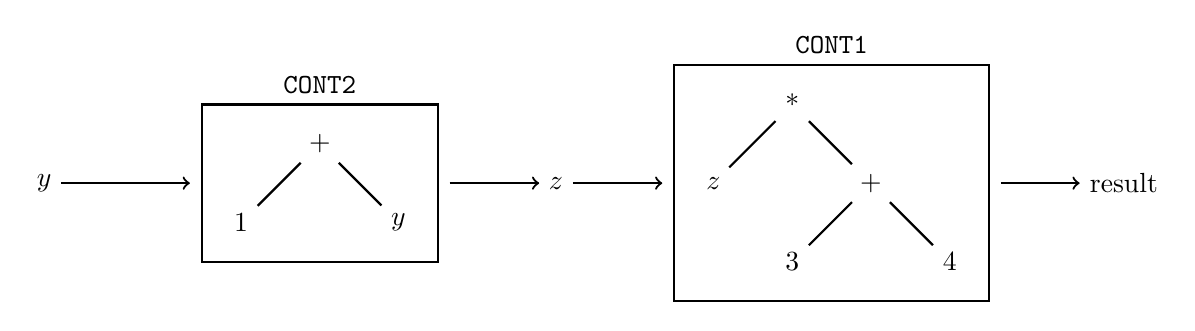
\begin{tikzpicture}
    \node (Y) at (0, -4) {$y$};
    \node (Z) at (6.5, -4) {$z$};
    \node (PLUS) at (3.5, -3.5) {+};
    \node (ONE) at (2.5, -4.5) {1};
    \node (Y2) at (4.5, -4.5) {$y$};

    \node (STAR) at (9.5, -3) {*};
    \node (Z2) at (8.5, -4) {$z$};
    \node (PLUS2) at (10.5, -4) {+};
    \node (THREE) at (9.5, -5) {3};
    \node (FOUR) at (11.5, -5) {4};

    \draw[->, black, thick] (Y) -- (1.85, -4);
    \draw[->, black, thick] (5.15, -4) -- (Z);
    \draw[->, black, thick] (Z) -- (7.85,-4);
    \draw[->, black, thick] (12.15, -4) -- (13.15,-4) node [at end, right] {result};
    
    \draw[black, thick] (ONE) -- (PLUS);
    \draw[black, thick] (PLUS) -- (Y2);

    \draw[black, thick] (PLUS2) -- (THREE);
    \draw[black, thick] (PLUS2) -- (FOUR);
    \draw[black, thick] (STAR) -- (PLUS2);
    \draw[black, thick] (STAR) -- (Z2);

    \draw[draw=black, thick] (2,-5) rectangle ++(3,2);
    \draw[draw=black, thick] (8,-5.5) rectangle ++(4,3);

    \node (CONT2) at (3.5, -2.75) {\texttt{CONT2}};
    \node (CONT1) at (10, -2.25) {\texttt{CONT1}};

    % \draw[->, red, thick] plot [smooth] coordinates {(4.25,-3.75) (3,-2) (5,-0.5) (7.25,-1.75)};
    
    % \draw[help lines] (0,0) grid (20,-20);
\end{tikzpicture}
\end{document}